\documentclass{article}
\usepackage{amsmath, amssymb, amscd, amsthm, amsfonts}
\usepackage{graphicx}
\usepackage{hyperref}
\usepackage{xcolor}
\usepackage{braket}
\usepackage{cancel}
\usepackage{float}

\oddsidemargin 0pt
\evensidemargin 0pt
\marginparwidth 40pt
\marginparsep 10pt
\topmargin -20pt
\headsep 10pt
\textheight 8.7in
\textwidth 6.65in
\linespread{1.2}

\title{PHYS401: Quantum Mechanics I \\ Homework \#10}
\author{Evan Shipley-Friedt}
\date{December 3rd, 2025}

% Extra spacing around equations
\setlength{\abovedisplayskip}{18pt}
\setlength{\belowdisplayskip}{18pt}
\setlength{\abovedisplayshortskip}{14pt}
\setlength{\belowdisplayshortskip}{14pt}

\begin{document}

\maketitle

{\huge Problem 1: Infinite Spherical Well ($\ell=0$)}

\section*{Solution}

\subsection*{(a) Normalized eigenstates and eigenvalues for $\ell=0$}

The potential is
\[
V(r)=
\begin{cases}
0, & 0\le r < a,\\
\infty, & r\ge a.
\end{cases}
\]
For $\ell=0$ (an $s$--state), the wavefunction separates as
\[
\psi(r,\theta,\phi)=R(r)\,Y_{00}(\theta,\phi),
\qquad
Y_{00}=\frac{1}{\sqrt{4\pi}}.
\]
Define the reduced radial function
\[
u(r)\equiv r\,R(r).
\]
For $\ell=0$ and $0<r<a$ (where $V=0$), the radial Schr\"odinger equation reduces to
\[
\frac{d^2u}{dr^2}+k^2u=0,
\qquad
k^2=\frac{2\mu E}{\hbar^2}.
\]
Regularity at $r=0$ requires $u(0)=0$, and the infinite wall at $r=a$ requires
\[
\psi(a)=0 \;\Rightarrow\; R(a)=0 \;\Rightarrow\; u(a)=0.
\]
The general solution is $u(r)=A\sin(kr)+B\cos(kr)$.  The condition $u(0)=0$ forces
$B=0$, so $u(r)=A\sin(kr)$.  The condition $u(a)=0$ gives
\[
\sin(ka)=0 \;\Rightarrow\; ka=n\pi,\qquad n=1,2,3,\dots
\]
Hence
\[
k_n=\frac{n\pi}{a},
\qquad
E_n=\frac{\hbar^2k_n^2}{2\mu}
=\frac{\hbar^2\pi^2}{2\mu a^2}\,n^2.
\]

Using the normalization identity for $\ell=0$,
\[
\int_0^a |u(r)|^2\,dr = 1,
\]
we obtain
\[
1=A^2\int_0^a \sin^2\!\left(\frac{n\pi r}{a}\right)\,dr
=A^2\frac{a}{2}
\;\Rightarrow\;
A=\sqrt{\frac{2}{a}}.
\]
Therefore the normalized reduced radial eigenfunctions are
\[
\boxed{
u_n(r)=\sqrt{\frac{2}{a}}\,
\sin\!\left(\frac{n\pi r}{a}\right)
\quad (0<r<a),
\qquad
u_n(r)=0\ (r\ge a)
}
\]
and
\[
\boxed{
R_n(r)=\frac{u_n(r)}{r}
=\sqrt{\frac{2}{a}}\,
\frac{\sin\!\left(\frac{n\pi r}{a}\right)}{r}
\quad (0<r<a),
\qquad
R_n(r)=0\ (r\ge a).
}
\]
The full (normalized) wavefunctions are
\[
\boxed{
\psi_{n00}(r,\theta,\phi)
=
R_n(r)\,Y_{00}(\theta,\phi)
=
\frac{1}{\sqrt{4\pi}}\sqrt{\frac{2}{a}}\,
\frac{\sin\!\left(\frac{n\pi r}{a}\right)}{r},
\quad (r<a),
\qquad
\psi_{n00}=0\ (r\ge a).
}
\]

\subsection*{(b) Plots of $P(r)=|u(r)|^2$ and $|R(r)|^2$ for the two lowest $s$--states}

For $\ell=0$, the radial probability in a shell $[r,r+dr]$ is
\[
\Pr(r\in[r,r+dr]) = |u(r)|^2\,dr,
\]
so $P(r)=|u(r)|^2$ is the physically relevant radial probability density in $r$.
The quantity $|R(r)|^2$ is shown as well for comparison.  On a log plot, true zeros
cannot be displayed; in the $|R(r)|^2$ plot a small display floor is used so that
zeros at nodes and at the wall appear consistently.

\begin{figure}[H]
\centering
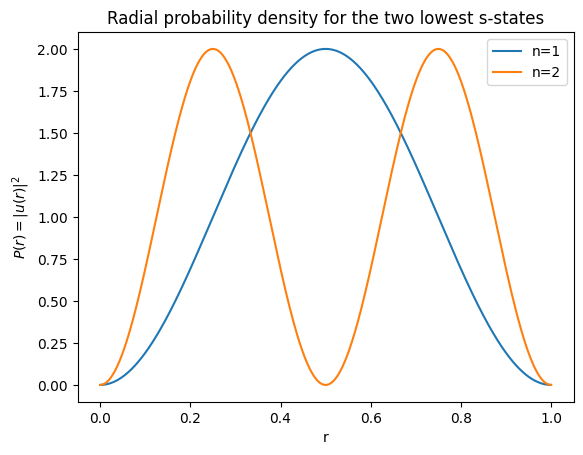
\includegraphics[width=0.85\textwidth]{well_P_u2.png}
\caption{Infinite spherical well ($\ell=0$): radial probability density $P(r)=|u(r)|^2$ for the two lowest states ($n=1,2$).}
\end{figure}

\begin{figure}[H]
\centering
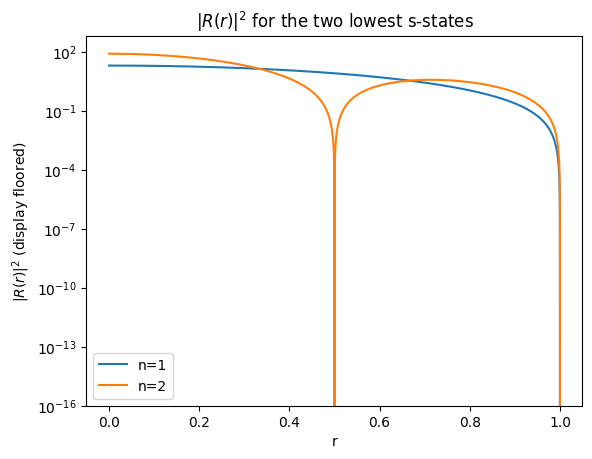
\includegraphics[width=0.85\textwidth]{well_R2.png}
\caption{Infinite spherical well ($\ell=0$): $|R(r)|^2$ for the two lowest states ($n=1,2$) on a log scale. Zeros at the node ($n=2$ at $r=a/2$) and at the wall ($r=a$) are displayed with a common floor for readability.}
\end{figure}

\subsection*{(c) How this differs from hydrogen $s$--states}

Although both problems involve $\ell=0$ ($s$--states), the physics and boundary
conditions are different:

\begin{itemize}
\item \textbf{Potential:} the spherical well has a hard wall at $r=a$, whereas hydrogen has a Coulomb potential
\[
V(r)=-\frac{e^2}{4\pi\varepsilon_0 r}
\]
with no finite boundary.
\item \textbf{Boundary condition at large $r$:} in the well, $u(a)=0$ forces the wavefunction to vanish at $r=a$ exactly.
In hydrogen, there is no wall; bound states satisfy normalizability, so the wavefunction decays smoothly as $r\to\infty$.
\item \textbf{Spectrum:} the well has $E_n\propto n^2$ (standing--wave quantization from the boundary),
while hydrogen has negative bound energies scaling like $E_n\propto -1/n^2$.
\item \textbf{Radial shapes:} in the well, $u_n(r)$ is sinusoidal.  In hydrogen, the $s$--state radial functions have
an exponential factor times a polynomial, producing nodes (e.g.\ the $2s$ node) without any hard wall.
\end{itemize}

For reference, the analogous plots for the hydrogen $1s$ and $2s$ states are shown below.

\begin{figure}[H]
\centering
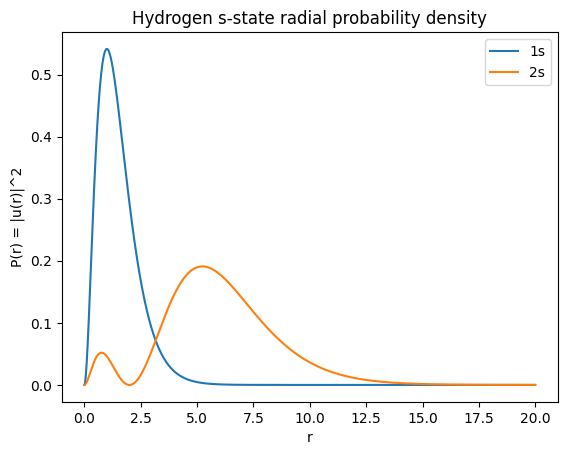
\includegraphics[width=0.85\textwidth]{hydrogen_P_u2.png}
\caption{Hydrogen atom: radial probability density $P(r)=|u(r)|^2$ for the $1s$ and $2s$ states. Unlike the spherical well, the distribution is not forced to vanish at a finite radius; it decays with an exponential tail.}
\end{figure}

\begin{figure}[H]
\centering
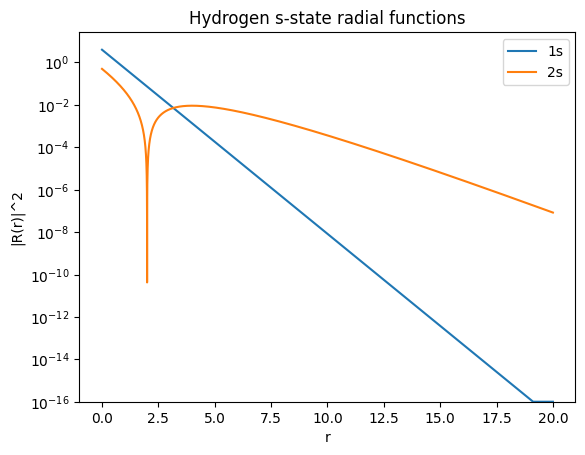
\includegraphics[width=0.85\textwidth]{hydrogen_R2.png}
\caption{Hydrogen atom: $|R(r)|^2$ for the $1s$ and $2s$ states on a log scale. The $2s$ node appears at a finite $r$, but there is no hard-wall boundary forcing $R(r)$ to vanish at a fixed radius.}
\end{figure}

\newpage

{\huge Problem 2: Sep. of Variables in Rect. Coords}

\section*{Solution}

\subsection*{(a) Derive the eigenstates and eigenvalues via separation of variables}

Inside the box ($0<x<a$, $0<y<b$, $0<z<c$) the potential is $V=0$, so the time--independent
Schr\"odinger equation (McIntyre Eq.~7.29) becomes
\[
-\frac{\hbar^2}{2m}\nabla^2\psi(x,y,z)=E\,\psi(x,y,z),
\qquad
\nabla^2=\frac{\partial^2}{\partial x^2}+\frac{\partial^2}{\partial y^2}+\frac{\partial^2}{\partial z^2}.
\]
Equivalently,
\[
\frac{\partial^2\psi}{\partial x^2}+\frac{\partial^2\psi}{\partial y^2}+\frac{\partial^2\psi}{\partial z^2}
+\frac{2mE}{\hbar^2}\psi=0.
\tag{1}
\]

We seek separated solutions of the form
\[
\psi(x,y,z)=X(x)\,Y(y)\,Z(z).
\]
Substituting into Eq.~(1) gives
\[
X''YZ + XY''Z + XYZ'' + \frac{2mE}{\hbar^2}XYZ = 0.
\]
Divide through by $XYZ$:
\[
\frac{X''}{X}+\frac{Y''}{Y}+\frac{Z''}{Z}+\frac{2mE}{\hbar^2}=0.
\tag{2}
\]
The first term depends only on $x$, the second only on $y$, and the third only on $z$,
so each must be equal to a constant.  Choose separation constants $k_x^2,k_y^2,k_z^2>0$
such that
\[
\frac{X''}{X}=-k_x^2,\qquad
\frac{Y''}{Y}=-k_y^2,\qquad
\frac{Z''}{Z}=-k_z^2,
\]
and therefore Eq.~(2) implies
\[
k_x^2+k_y^2+k_z^2=\frac{2mE}{\hbar^2}.
\tag{3}
\]
This yields three ordinary differential equations:
\[
X''+k_x^2X=0,\qquad
Y''+k_y^2Y=0,\qquad
Z''+k_z^2Z=0.
\tag{4}
\]
These are exactly the same form as the 1D infinite square well (Ch.~5).

Because the potential is infinite outside the region, the wavefunction must vanish
on each boundary:
\[
\psi(0,y,z)=\psi(a,y,z)=0,\quad
\psi(x,0,z)=\psi(x,b,z)=0,\quad
\psi(x,y,0)=\psi(x,y,c)=0.
\]
For separated solutions this implies
\[
X(0)=X(a)=0,\qquad Y(0)=Y(b)=0,\qquad Z(0)=Z(c)=0.
\tag{5}
\]

Solving $X''+k_x^2X=0$ gives $X=A\sin(k_x x)+B\cos(k_x x)$.
The condition $X(0)=0$ forces $B=0$, and $X(a)=0$ requires
\[
\sin(k_x a)=0 \;\Rightarrow\; k_x a = n_x\pi,\qquad n_x=1,2,3,\dots
\]
so
\[
k_x=\frac{n_x\pi}{a},\qquad X_{n_x}(x)=A\sin\!\left(\frac{n_x\pi x}{a}\right).
\]
\[
k_y=\frac{n_y\pi}{b},\qquad Y_{n_y}(y)=C\sin\!\left(\frac{n_y\pi y}{b}\right),
\]
\[
k_z=\frac{n_z\pi}{c},\qquad Z_{n_z}(z)=D\sin\!\left(\frac{n_z\pi z}{c}\right),
\]
with $n_y,n_z=1,2,3,\dots$

Using Eq.~(3), the energy is
\[
E=\frac{\hbar^2}{2m}\left(k_x^2+k_y^2+k_z^2\right)
=\frac{\hbar^2}{2m}\left(\frac{n_x^2\pi^2}{a^2}+\frac{n_y^2\pi^2}{b^2}+\frac{n_z^2\pi^2}{c^2}\right).
\]
Thus,
\[
\boxed{
E_{n_x n_y n_z}
=
\frac{\hbar^2\pi^2}{2m}
\left(
\frac{n_x^2}{a^2}+\frac{n_y^2}{b^2}+\frac{n_z^2}{c^2}
\right)
}
\qquad (n_x,n_y,n_z\in\mathbb{Z}^+).
\]

Finally, normalize the eigenfunction.  Because the variables separate,
\[
1=\int_0^a\int_0^b\int_0^c |\psi|^2\,dx\,dy\,dz
=\left(\int_0^a |X|^2dx\right)\left(\int_0^b |Y|^2dy\right)\left(\int_0^c |Z|^2dz\right).
\]
Using the standard 1D result
\[
\int_0^a \sin^2\!\left(\frac{n\pi x}{a}\right)\,dx=\frac{a}{2},
\]
we choose $A=\sqrt{2/a}$, $C=\sqrt{2/b}$, $D=\sqrt{2/c}$. Therefore the normalized
stationary states are
\[
\boxed{
\phi_{n_x n_y n_z}(x,y,z)
=
\sqrt{\frac{2}{a}}\sqrt{\frac{2}{b}}\sqrt{\frac{2}{c}}\,
\sin\!\left(\frac{n_x\pi x}{a}\right)
\sin\!\left(\frac{n_y\pi y}{b}\right)
\sin\!\left(\frac{n_z\pi z}{c}\right)
}
\]
for $0<x<a$, $0<y<b$, $0<z<c$, and $\phi=0$ otherwise.

\subsection*{(b) Lowest 4 distinct energy levels for $b=c=\sqrt{2}\,a$}

From part (a),
\[
E_{n_x n_y n_z}
=
\frac{\hbar^2\pi^2}{2m}
\left(
\frac{n_x^2}{a^2}+\frac{n_y^2}{b^2}+\frac{n_z^2}{c^2}
\right).
\]
With
\[
b=\sqrt{2}\,a,\qquad c=\sqrt{2}\,a,
\]
we have $b^2=c^2=2a^2$, so
\[
E_{n_x n_y n_z}
=
\frac{\hbar^2\pi^2}{2m a^2}
\left(
n_x^2+\frac{n_y^2}{2}+\frac{n_z^2}{2}
\right)
=
\frac{\hbar^2\pi^2}{4m a^2}\,
\underbrace{\left(2n_x^2+n_y^2+n_z^2\right)}_{\equiv\,Q}.
\tag{6}
\]
Thus distinct energies correspond to distinct integer values of
\[
Q=2n_x^2+n_y^2+n_z^2,\qquad n_x,n_y,n_z=1,2,3,\dots
\]
We now list the smallest values of $Q$ and the corresponding quantum numbers.

\begin{itemize}
\item \textbf{Ground level:} $(n_x,n_y,n_z)=(1,1,1)$ gives
\[
Q=2(1)^2+1^2+1^2=4
\quad\Rightarrow\quad
E_1=\frac{\hbar^2\pi^2}{4ma^2}(4)=\frac{\hbar^2\pi^2}{ma^2}.
\]

\item \textbf{Second distinct level:} $(1,1,2)$ and $(1,2,1)$ give
\[
Q=2(1)^2+1^2+2^2=7
\quad\Rightarrow\quad
E_2=\frac{\hbar^2\pi^2}{4ma^2}(7)=\frac{7}{4}\frac{\hbar^2\pi^2}{ma^2}.
\]

\item \textbf{Third distinct level:} $(1,2,2)$ and $(2,1,1)$ give
\[
Q=2(1)^2+2^2+2^2=10,
\qquad
Q=2(2)^2+1^2+1^2=10,
\]
so both correspond to
\[
E_3=\frac{\hbar^2\pi^2}{4ma^2}(10)=\frac{5}{2}\frac{\hbar^2\pi^2}{ma^2}.
\]

\item \textbf{Fourth distinct level:} $(1,1,3)$ and $(1,3,1)$ give
\[
Q=2(1)^2+1^2+3^2=12
\quad\Rightarrow\quad
E_4=\frac{\hbar^2\pi^2}{4ma^2}(12)=3\,\frac{\hbar^2\pi^2}{ma^2}.
\]
\end{itemize}

\subsection*{(c) Degeneracies of the levels}

Because $b=c$, the Hamiltonian is symmetric under interchange $y\leftrightarrow z$.
Therefore, whenever $n_y\neq n_z$, the two states $(n_x,n_y,n_z)$ and $(n_x,n_z,n_y)$
have the same energy, giving at least a twofold degeneracy. In addition, there can be
``accidental'' degeneracy when different triples produce the same value of
$Q=2n_x^2+n_y^2+n_z^2$.

For the four lowest distinct levels found above:

\begin{itemize}
\item $E_1$ (from $(1,1,1)$): degeneracy $g_1=1$.
\item $E_2$ (from $(1,1,2)$ and $(1,2,1)$): degeneracy $g_2=2$ (swap $y$ and $z$).
\item $E_3$ (from $(1,2,2)$ and $(2,1,1)$): degeneracy $g_3=2$ (accidental degeneracy).
\item $E_4$ (from $(1,1,3)$ and $(1,3,1)$): degeneracy $g_4=2$ (swap $y$ and $z$).
\end{itemize}

\newpage

{\huge Problem 3: Angular Momentum Kets Practice}

\section*{Solution}

We are given the state at $t=0$,
\[
\ket{\psi(0)}
=
\frac{1}{\sqrt{12}}\ket{0,0}
+
\frac{\sqrt{2}}{\sqrt{12}}\ket{1,-1}
+
\frac{3}{\sqrt{12}}\ket{1,0},
\]
where $\ket{\ell,m}$ are simultaneous eigenstates of $L^2$ and $L_z$:
\[
L_z\ket{\ell,m}=\hbar m\ket{\ell,m},\qquad
L^2\ket{\ell,m}=\hbar^2\ell(\ell+1)\ket{\ell,m}.
\]
The state is normalized since
\[
\frac{1}{12}+\frac{2}{12}+\frac{9}{12}=1.
\]

\subsection*{(a) Measurement of $L_z$}

A measurement of $L_z$ yields eigenvalues $\hbar m$ corresponding to the $m$ values
present in the state.

\begin{itemize}
\item $m=0$ arises from both $\ket{0,0}$ and $\ket{1,0}$:
\[
P(L_z=0)
=
\left|\frac{1}{\sqrt{12}}\right|^2
+
\left|\frac{3}{\sqrt{12}}\right|^2
=
\frac{1}{12}+\frac{9}{12}
=
\frac{5}{6}.
\]

\item $m=-1$ arises from $\ket{1,-1}$:
\[
P(L_z=-\hbar)
=
\left|\frac{\sqrt{2}}{\sqrt{12}}\right|^2
=
\frac{2}{12}
=
\frac{1}{6}.
\]
\end{itemize}

There is no $\ket{1,+1}$ component, so $P(L_z=+\hbar)=0$.

\subsection*{(b) Measurement of $L^2$}

A measurement of $L^2$ yields eigenvalues $\hbar^2\ell(\ell+1)$.

\begin{itemize}
\item $\ell=0 \Rightarrow L^2=0$:
\[
P(L^2=0)
=
\left|\frac{1}{\sqrt{12}}\right|^2
=
\frac{1}{12}.
\]

\item $\ell=1 \Rightarrow L^2=2\hbar^2$:
\[
P(L^2=2\hbar^2)
=
\left|\frac{\sqrt{2}}{\sqrt{12}}\right|^2
+
\left|\frac{3}{\sqrt{12}}\right|^2
=
\frac{2}{12}+\frac{9}{12}
=
\frac{11}{12}.
\]
\end{itemize}

\subsection*{(c) Measure $L_z=-\hbar$, then measure $L_x$ (using McIntyre spin--1 results)}

If the measurement of $L_z$ yields $-\hbar$, the state collapses onto the corresponding
$L_z$ eigenket in the $\ell=1$ subspace:
\[
\ket{\psi}\;\longrightarrow\;\ket{1,-1}.
\]
For $\ell=1$ (a spin--1 system), the possible outcomes of measuring $L_x$ are
\[
L_x = \hbar m_x,\qquad m_x\in\{+1,0,-1\}.
\]

McIntyre (spin--1 system) gives the $S_x$ eigenkets written in the $S_z$ basis as:
\[
\ket{+1}_x = \frac{1}{2}\ket{+1}+\frac{1}{\sqrt2}\ket{0}+\frac{1}{2}\ket{-1},
\]
\[
\ket{0}_x = \frac{1}{\sqrt2}\ket{+1}-\frac{1}{\sqrt2}\ket{-1},
\]
\[
\ket{-1}_x = \frac{1}{2}\ket{+1}-\frac{1}{\sqrt2}\ket{0}+\frac{1}{2}\ket{-1}.
\]
Here we identify $\ket{+1}\equiv\ket{1,+1}$, $\ket{0}\equiv\ket{1,0}$, and
$\ket{-1}\equiv\ket{1,-1}$ (McIntyre's notation).

We want the probabilities for outcomes of $L_x$ when the system is in the state $\ket{-1}$.
Using the projection postulate,
\[
P(m_x)=|\braket{m_x{}_x|-1}|^2.
\]

Compute the overlaps by taking inner products with $\ket{-1}$:

\begin{align*}
\braket{+1_x|-1}
&=
\left(\frac{1}{2}\bra{+1}+\frac{1}{\sqrt2}\bra{0}+\frac{1}{2}\bra{-1}\right)\ket{-1}
= \frac{1}{2}\braket{-1|-1}
= \frac{1}{2},\\[6pt]
\braket{0_x|-1}
&=
\left(\frac{1}{\sqrt2}\bra{+1}-\frac{1}{\sqrt2}\bra{-1}\right)\ket{-1}
= -\frac{1}{\sqrt2}\braket{-1|-1}
= -\frac{1}{\sqrt2},\\[6pt]
\braket{-1_x|-1}
&=
\left(\frac{1}{2}\bra{+1}-\frac{1}{\sqrt2}\bra{0}+\frac{1}{2}\bra{-1}\right)\ket{-1}
= \frac{1}{2}\braket{-1|-1}
= \frac{1}{2}.
\end{align*}

Therefore the probabilities are
\[
P(m_x=+1)=\left|\frac{1}{2}\right|^2=\frac{1}{4},\qquad
P(m_x=0)=\left|\frac{1}{\sqrt2}\right|^2=\frac{1}{2},\qquad
P(m_x=-1)=\left|\frac{1}{2}\right|^2=\frac{1}{4}.
\]
Thus the possible measurement results for $L_x$ are
\[
\boxed{
L_x=+\hbar\ (1/4),\qquad
L_x=0\ (1/2),\qquad
L_x=-\hbar\ (1/4).
}
\]

\newpage

\subsection*{(d) Measure $L^2=2\hbar^2$}

\subsubsection*{(i) New state after the measurement}

Measuring $L^2$ and obtaining $2\hbar^2$ projects the state onto the $\ell=1$ subspace.
The unnormalized projected state is
\[
\ket{\psi_{\ell=1}}
=
\frac{\sqrt{2}}{\sqrt{12}}\ket{1,-1}
+
\frac{3}{\sqrt{12}}\ket{1,0}.
\]
Its norm squared is
\[
\frac{2}{12}+\frac{9}{12}=\frac{11}{12},
\]
so the normalized post--measurement state is
\[
\boxed{
\ket{\psi'}
=
\sqrt{\frac{2}{11}}\ket{1,-1}
+
\frac{3}{\sqrt{11}}\ket{1,0}
}.
\]

\subsubsection*{(ii) Measure $L_z$ after measuring $L^2$}

In the state $\ket{\psi'}$, the possible $L_z$ outcomes are
\[
L_z=-\hbar \quad \text{and} \quad L_z=0.
\]
The probabilities are
\[
P(L_z=-\hbar)=\left|\sqrt{\frac{2}{11}}\right|^2=\frac{2}{11},\qquad
P(L_z=0)=\left|\frac{3}{\sqrt{11}}\right|^2=\frac{9}{11}.
\]
There is no $m=+1$ component, so $P(L_z=+\hbar)=0$.

\newpage

{\huge Problem 4: Particle on a Ring}

\section*{Solution}

A particle of mass $\mu$ constrained to a ring of radius $a$ has
\[
\hat H=\frac{\hat L_z^{\,2}}{2\mu a^2}.
\]
In lecture, simultaneous eigenkets of $\hat H$ and $\hat L_z$ were denoted $\ket{m}$, with
\[
\hat L_z\ket{m}=\hbar m\ket{m},
\qquad
\hat H\ket{m}=E_m\ket{m},
\qquad
E_m=\frac{\hbar^2 m^2}{2\mu a^2}.
\]
The initial state is
\[
\ket{\psi(0)}
=\frac{2}{5}\ket{-3}
+\frac{2\sqrt{3}}{5}\ket{+1}
+\frac{3}{5}\ket{+3}.
\]
It is normalized since
\[
\left|\frac{2}{5}\right|^2+\left|\frac{2\sqrt3}{5}\right|^2+\left|\frac{3}{5}\right|^2
=\frac{4}{25}+\frac{12}{25}+\frac{9}{25}=1.
\]

\subsection*{(a) Measure $L_z$}

The possible results are the eigenvalues $\hbar m$ appearing in the expansion.

\[
P(L_z=-3\hbar)=\left|\frac{2}{5}\right|^2=\frac{4}{25},
\qquad
P(L_z=+\hbar)=\left|\frac{2\sqrt3}{5}\right|^2=\frac{12}{25},
\qquad
P(L_z=+3\hbar)=\left|\frac{3}{5}\right|^2=\frac{9}{25}.
\]

\subsection*{(b) Measure energy}

Since $E_m=\hbar^2 m^2/(2\mu a^2)$, the distinct energies present are:

\begin{itemize}
\item For $m=+1$:
\[
E_1=\frac{\hbar^2}{2\mu a^2},
\qquad
P(E_1)=\frac{12}{25}.
\]
\item For $m=\pm 3$:
\[
E_3=\frac{9\hbar^2}{2\mu a^2},
\qquad
P(E_3)=P(m=-3)+P(m=+3)=\frac{4}{25}+\frac{9}{25}=\frac{13}{25}.
\]
\end{itemize}

\subsection*{(c) Compute $\langle \hat L_z\rangle$ and $\langle \hat H\rangle$}

Using $\langle \hat L_z\rangle=\sum_m |c_m|^2(\hbar m)$:
\[
\langle \hat L_z\rangle
=\hbar\left[(-3)\frac{4}{25}+(1)\frac{12}{25}+(3)\frac{9}{25}\right]
=\hbar\left(\frac{-12+12+27}{25}\right)
=
\boxed{\frac{27}{25}\hbar}.
\]

Using $\langle \hat H\rangle=\sum_m |c_m|^2\,\hbar^2 m^2/(2\mu a^2)$:
\[
\langle \hat H\rangle
=\frac{\hbar^2}{2\mu a^2}\left[9\frac{4}{25}+1\frac{12}{25}+9\frac{9}{25}\right]
=\frac{\hbar^2}{2\mu a^2}\left(\frac{36+12+81}{25}\right)
=
\boxed{\frac{129}{25}\,\frac{\hbar^2}{2\mu a^2}}.
\]

\subsection*{(d) First measure $L_z=+\hbar$, then measure energy}

If the first measurement yields $L_z=+\hbar$, then the state collapses to the corresponding
eigenket:
\[
\ket{\psi}\longrightarrow \ket{+1}.
\]
But $\ket{+1}$ is also an energy eigenstate (since $\hat H$ and $\hat L_z$ share eigenkets),
with
\[
\hat H\ket{+1}=\frac{\hbar^2}{2\mu a^2}\ket{+1}.
\]
Therefore the subsequent energy measurement is certain:
\[
\boxed{
E=\frac{\hbar^2}{2\mu a^2}\ \ \text{with probability }1.
}
\]

\subsection*{(e) First measure $E=\dfrac{9\hbar^2}{2\mu a^2}$, then measure $L_z$}

The energy $E=\dfrac{9\hbar^2}{2\mu a^2}$ corresponds to $m^2=9$, i.e.\ the degenerate
subspace spanned by $\{\ket{-3},\ket{+3}\}$. Measuring this energy projects the state onto
that subspace:
\[
\ket{\psi}\ \longrightarrow\
\ket{\psi_E}
\propto
\frac{2}{5}\ket{-3}+\frac{3}{5}\ket{+3}.
\]
The norm squared of the projected part is
\[
\left|\frac{2}{5}\right|^2+\left|\frac{3}{5}\right|^2=\frac{4}{25}+\frac{9}{25}=\frac{13}{25},
\]
so
\[
\boxed{
\ket{\psi_E}
=
\sqrt{\frac{4}{13}}\ket{-3}
+
\sqrt{\frac{9}{13}}\ket{+3}
=
\frac{2}{\sqrt{13}}\ket{-3}+\frac{3}{\sqrt{13}}\ket{+3}.
}
\]
Now measure $L_z$ in this state. The possible outcomes are $L_z=\pm 3\hbar$ with
probabilities given by the squared amplitudes:
\[
\boxed{
P(L_z=-3\hbar)=\left|\frac{2}{\sqrt{13}}\right|^2=\frac{4}{13},
\qquad
P(L_z=+3\hbar)=\left|\frac{3}{\sqrt{13}}\right|^2=\frac{9}{13}.
}
\]

\newpage

{\huge Problem 6: Particle on a Sphere}

\section*{Solution}

We are given the spherical harmonic (in position space)
\[
\ket{1,-1}\ \widehat{=}\ Y_1^{-1}(\theta,\phi)
=
\sqrt{\frac{3}{8\pi}}\;\sin\theta\;e^{-i\phi}.
\]
Recall the standard angular momentum eigenvalue equations,
\[
\hat L_z Y_\ell^{m} = \hbar m\,Y_\ell^{m},
\qquad
\hat L^2 Y_\ell^{m} = \hbar^2\ell(\ell+1)\,Y_\ell^{m}.
\]

\subsection*{(a) Act with $L_z$ and find the eigenvalue}

In spherical coordinates, the $z$--component of orbital angular momentum in position space is
\[
\hat L_z=-i\hbar\frac{\partial}{\partial\phi}.
\]
Acting on $Y_1^{-1}(\theta,\phi)$:
\begin{align*}
\hat L_z\,Y_1^{-1}
&=
-i\hbar\frac{\partial}{\partial\phi}
\left(
\sqrt{\frac{3}{8\pi}}\sin\theta\,e^{-i\phi}
\right)\\[4pt]
&=
-i\hbar\left(
\sqrt{\frac{3}{8\pi}}\sin\theta
\right)\left(-i e^{-i\phi}\right)\\[4pt]
&=
(-\hbar)\,
\sqrt{\frac{3}{8\pi}}\sin\theta\,e^{-i\phi}\\[4pt]
&=
-\hbar\,Y_1^{-1}(\theta,\phi).
\end{align*}
Therefore,
\[
\boxed{\ \hat L_z\,Y_1^{-1} = (-\hbar)\,Y_1^{-1}\ }
\]
so the eigenvalue is $m\hbar$ with $m=-1$, as expected from $\ket{\ell=1,m=-1}$.

\subsection*{(b) Act with $L^2$ and find the eigenvalue}

A defining property of spherical harmonics is
\[
\hat L^2\,Y_\ell^{m}=\hbar^2\ell(\ell+1)\,Y_\ell^{m}.
\]
For $\ell=1$ this gives
\[
\boxed{\ \hat L^2\,Y_1^{-1}= \hbar^2(1)(2)\,Y_1^{-1}=2\hbar^2\,Y_1^{-1}\ }.
\]
So the eigenvalue of $L^2$ is $2\hbar^2$.

\subsection*{(c) Verify normalization on the unit sphere}

Normalization over the surface of the unit sphere means
\[
\int_0^{2\pi}\int_0^\pi |Y_1^{-1}(\theta,\phi)|^2\,\sin\theta\,d\theta\,d\phi = 1,
\qquad d\Omega=\sin\theta\,d\theta\,d\phi.
\]
Compute the magnitude squared:
\[
|Y_1^{-1}|^2
=
\left(\sqrt{\frac{3}{8\pi}}\right)^2
\sin^2\theta\;|e^{-i\phi}|^2
=
\frac{3}{8\pi}\sin^2\theta,
\]
since $|e^{-i\phi}|^2=1$. Then
\begin{align*}
\int |Y_1^{-1}|^2\,d\Omega
&=
\int_0^{2\pi}\int_0^\pi
\frac{3}{8\pi}\sin^2\theta\;\sin\theta\,d\theta\,d\phi\\[4pt]
&=
\frac{3}{8\pi}\left(\int_0^{2\pi}d\phi\right)
\left(\int_0^\pi \sin^3\theta\,d\theta\right)\\[4pt]
&=
\frac{3}{8\pi}(2\pi)\left(\int_0^\pi \sin^3\theta\,d\theta\right)\\[4pt]
&=
\frac{3}{4}\left(\int_0^\pi \sin^3\theta\,d\theta\right).
\end{align*}
Using the standard result
\[
\int_0^\pi \sin^3\theta\,d\theta=\frac{4}{3},
\]
we obtain
\[
\frac{3}{4}\cdot\frac{4}{3}=1.
\]
Hence,
\[
\boxed{\ \int_0^{2\pi}\int_0^\pi |Y_1^{-1}(\theta,\phi)|^2\,\sin\theta\,d\theta\,d\phi = 1\ },
\]
so the function is correctly normalized over the unit sphere.

\subsection*{(d) What can we infer from Fig.~7.19 about probability?}

Figure~7.19 shows 3D polar plots of $|Y_\ell^m(\theta,\phi)|^2$, i.e.\ the \emph{angular}
probability density as a function of direction $(\theta,\phi)$.  For our state,
\[
|Y_1^{-1}(\theta,\phi)|^2=\frac{3}{8\pi}\sin^2\theta,
\]
which is independent of $\phi$. Therefore the probability is
\begin{itemize}
\item \textbf{maximal at the equator} ($\theta=\pi/2$), since $\sin^2(\pi/2)=1$,
\item \textbf{zero at the poles} ($\theta=0,\pi$), since $\sin^2(0)=\sin^2(\pi)=0$.
\end{itemize}
This matches the torus--like (donut) shape shown in Fig.~7.19 for $|Y_1^{\pm 1}|^2$:
the particle is most likely to be found near the equatorial directions and least likely
to be found along the $\pm z$ axis.

\newpage

{\huge Problem 7: Spherical Harmonics Decomposition}

\section*{Solution}

A particle confined to the surface of a sphere is in the state
\[
\psi(\theta,\phi)=
\begin{cases}
N\left(\dfrac{\pi^2}{4}-\theta^2\right), & 0<\theta\le \dfrac{\pi}{2},\\[8pt]
0, & \dfrac{\pi}{2}<\theta<\pi,
\end{cases}
\]
(where $N$ is given in the problem).  Since the particle is on the sphere, the inner product is
\[
\braket{f|g}=\int_0^{2\pi}\!\!\int_0^\pi f^*(\theta,\phi)\,g(\theta,\phi)\,\sin\theta\,d\theta\,d\phi
\equiv \int f^* g\,d\Omega.
\]
We expand in spherical harmonics:
\[
\psi(\theta,\phi)=\sum_{\ell=0}^\infty\sum_{m=-\ell}^{\ell} c_{\ell m}\,Y_\ell^m(\theta,\phi),
\qquad
c_{\ell m}=\int \psi(\theta,\phi)\,Y_\ell^{m*}(\theta,\phi)\,d\Omega.
\]

\subsection*{(a) Coefficients for $\ket{0,0}$, $\ket{1,-1}$, $\ket{1,0}$, $\ket{1,1}$}

Because $\psi(\theta,\phi)$ is independent of $\phi$, the $\phi$--integral forces $m=0$.
In particular, for $m\neq 0$ the spherical harmonics contain $e^{im\phi}$, and
\[
\int_0^{2\pi} e^{-im\phi}\,d\phi = 0\quad (m\neq 0),
\]
so
\[
\boxed{c_{1,-1}=0,\qquad c_{1,1}=0.}
\]

We now compute $c_{00}$ and $c_{10}$.  Using
\[
Y_0^0=\frac{1}{\sqrt{4\pi}},\qquad
Y_1^0=\sqrt{\frac{3}{4\pi}}\cos\theta,
\]
and the fact that $\psi$ is nonzero only on $0\le\theta\le\pi/2$:

\medskip
\noindent\textbf{Coefficient $c_{00}$.}
\begin{align*}
c_{00}
&=\int \psi\,Y_0^{0*}\,d\Omega\\
&=\int_0^{2\pi}\!\!\int_0^{\pi/2}
N\left(\frac{\pi^2}{4}-\theta^2\right)\left(\frac{1}{\sqrt{4\pi}}\right)\sin\theta\,d\theta\,d\phi\\
&=\frac{2\pi N}{\sqrt{4\pi}}
\int_0^{\pi/2}\left(\frac{\pi^2}{4}-\theta^2\right)\sin\theta\,d\theta.
\end{align*}
The integral evaluates to
\[
\int_0^{\pi/2}\left(\frac{\pi^2}{4}-\theta^2\right)\sin\theta\,d\theta
=
-\pi+2+\frac{\pi^2}{4}.
\]
Also $\dfrac{2\pi}{\sqrt{4\pi}}=\sqrt{\pi}$, so
\[
\boxed{
c_{00}=N\sqrt{\pi}\left(-\pi+2+\frac{\pi^2}{4}\right).
}
\]

\medskip
\noindent\textbf{Coefficient $c_{10}$.}
\begin{align*}
c_{10}
&=\int \psi\,Y_1^{0*}\,d\Omega\\
&=\int_0^{2\pi}\!\!\int_0^{\pi/2}
N\left(\frac{\pi^2}{4}-\theta^2\right)\left(\sqrt{\frac{3}{4\pi}}\cos\theta\right)\sin\theta\,d\theta\,d\phi\\
&=2\pi N\sqrt{\frac{3}{4\pi}}
\int_0^{\pi/2}\left(\frac{\pi^2}{4}-\theta^2\right)\sin\theta\cos\theta\,d\theta.
\end{align*}
The integral evaluates to
\[
\int_0^{\pi/2}\left(\frac{\pi^2}{4}-\theta^2\right)\sin\theta\cos\theta\,d\theta
=
\frac{1}{4}+\frac{\pi^2}{16}
=\frac{4+\pi^2}{16}.
\]
Also $2\pi\sqrt{\dfrac{3}{4\pi}}=\sqrt{3\pi}$, so
\[
\boxed{
c_{10}=N\sqrt{3\pi}\;\frac{4+\pi^2}{16}.
}
\]

Collecting the four requested coefficients:
\[
\boxed{
c_{00}=N\sqrt{\pi}\left(-\pi+2+\frac{\pi^2}{4}\right),\quad
c_{1,-1}=0,\quad
c_{10}=N\sqrt{3\pi}\;\frac{4+\pi^2}{16},\quad
c_{1,1}=0.
}
\]

\subsection*{(b) Probabilities for a measurement of $L^2$}

On a sphere, the spherical harmonics are eigenstates of $L^2$:
\[
\hat L^2 Y_\ell^m = \hbar^2\ell(\ell+1)Y_\ell^m.
\]
Thus:
\[
\ell=0 \Rightarrow L^2=0,\qquad
\ell=1 \Rightarrow L^2=2\hbar^2.
\]
Using only the coefficients found in (a),
\[
\boxed{
P(L^2=0)=|c_{00}|^2,
\qquad
P(L^2=2\hbar^2)=\sum_{m=-1}^1 |c_{1m}|^2 = |c_{10}|^2.
}
\]
Explicitly,
\[
\boxed{
P(L^2=0)=
N^2\pi\left(-\pi+2+\frac{\pi^2}{4}\right)^2,
\qquad
P(L^2=2\hbar^2)=
N^2\,3\pi\left(\frac{4+\pi^2}{16}\right)^2.
}
\]
(Note: because $\psi$ is not exactly a linear combination of only $\ell=0,1$ harmonics, the
remaining probability lies in $\ell\ge 2$ terms that are being neglected in this approximation.)

\subsection*{(c) Approximate time-dependent wavefunction using the terms in (a)}

The Hamiltonian is given by
\[
H_{\text{sphere}}Y_\ell^m(\theta,\phi)=\frac{\hbar^2}{2I}\,\ell(\ell+1)\,Y_\ell^m(\theta,\phi),
\]
so the energy eigenvalues are
\[
E_\ell=\frac{\hbar^2}{2I}\ell(\ell+1).
\]
Therefore
\[
E_0=0,\qquad
E_1=\frac{\hbar^2}{2I}\cdot 2=\frac{\hbar^2}{I}.
\]
Keeping only the $\ell=0$ and $\ell=1$ pieces found in (a), the approximate time-dependent
wavefunction is
\[
\boxed{
\psi(\theta,\phi,t)\approx
c_{00}\,Y_0^0(\theta,\phi)\,e^{-iE_0 t/\hbar}
+
c_{10}\,Y_1^0(\theta,\phi)\,e^{-iE_1 t/\hbar}
}
\]
i.e.
\[
\boxed{
\psi(\theta,\phi,t)\approx
c_{00}\,Y_0^0(\theta,\phi)
+
c_{10}\,Y_1^0(\theta,\phi)\,e^{-i(\hbar/I)t},
}
\]
with $c_{00}$ and $c_{10}$ given above.

\newpage

\end{document}